\subsection{Bedrock Geology}\label{subsec:bedrock}
\subsection*{Why you need this map}
A region's landscape is greatly influenced by its geology and the processes 
which modify it. The Hudson Valley’s diverse geology contributes to our local 
ecosystems and enables many human activities and industries as well. Gypsum and 
limestone deposits along the Hudson River support cement factories, shale and 
sand and gravel mines dot the valley’s landscape, the "black dirt" region’s 
fertile soils support agriculture, and mountain ridges and other geologic 
features are popular destinations for outdoor recreation. Bedrock and surficial 
geology strongly influence soil properties as well as groundwater and surface 
water chemistry, which in turn influence the type of ecological communities that 
can thrive ~\citep{haeckel2014}. More detailed information of the different types 
of soils found in Cornwall is available in the General Soil Classes chapter of 
this \gls{nri}.

Bedrock is solid rock that typically lies beneath soil and other broken or 
unconsolidated material (regolith). Bedrock is made up of igneous, sedimentary, 
or metamorphic rock, and it often serves as the parent material for regolith 
and soil. A bedrock deposit that occurs at Earth’s surface is called an 
outcrop. The processes of weathering and erosion affect bedrock. Outcrops 
exposed to wind and water are often decomposed, or weathered, over time into 
regolith or smaller particles.1 Knowledge of regional bedrock characteristics is 
important to planning, as it plays an important part in determining the 
viability of well water access and productivity, and large scale slope and grade 
stabilization. More detailed information about Cornwall's wells and aquifers can 
be found in the ~\nameref{subsec:groundwater} section of this NRI.

\begin{figure}
  \begin{centering}
    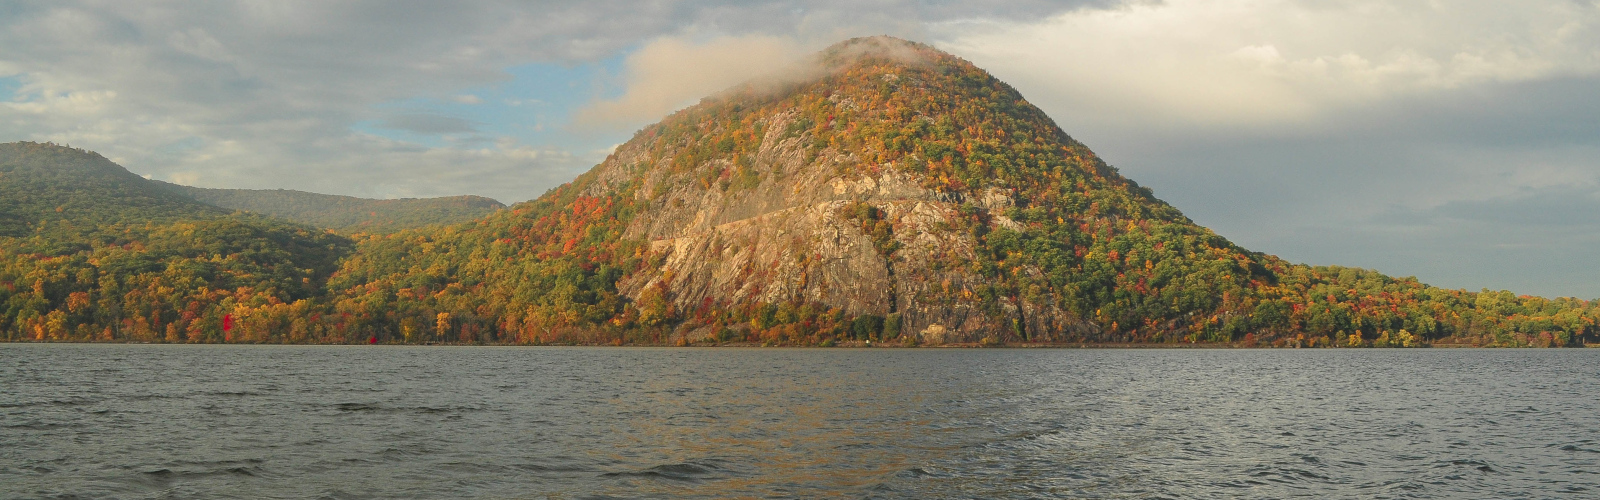
\includegraphics[width=\textwidth]{images/stormking.jpg}
    \vspace{-10pt}
    \caption{Storm King Mountain}\label{fig:stormking}
  \end{centering}
\end{figure}

Surficial geology is the study of landforms and the geologic materials lying on 
top of the bedrock. These materials can be sand and gravel, clay and silts, and 
glacial tills. Mapping these glacial deposits and other aspects of surficial 
geology provides important information to aid land use decisions, such as 
building roads and other structures; safeguarding drinking water; preparing for 
natural disasters; protecting wildlife and their habitats; and mitigating the 
effects of geologic hazards. Such information benefits residents and industry 
alike.

\includepdf[pages=-,fitpaper]{cornwall_maps/BedrockGeology.pdf}\label{map:bedrockgeology}

\subsection*{Bedrock and Surficial Geology of the Town of Cornwall and the 
Village of Cornwall-on-Hudson}
Cornwall has its share of stunning magnificent granite outcroppings in Storm 
King State Park that have captured the imagination of settlers, rusticators, 
and tourists for generations. This map identifies the four main types of 
bedrock to be found in the Town of Cornwall and Village.
\vspace{4mm}
%0.4\textwidth
\begin{wrapfigure}{r}{0pt}
    \centering
        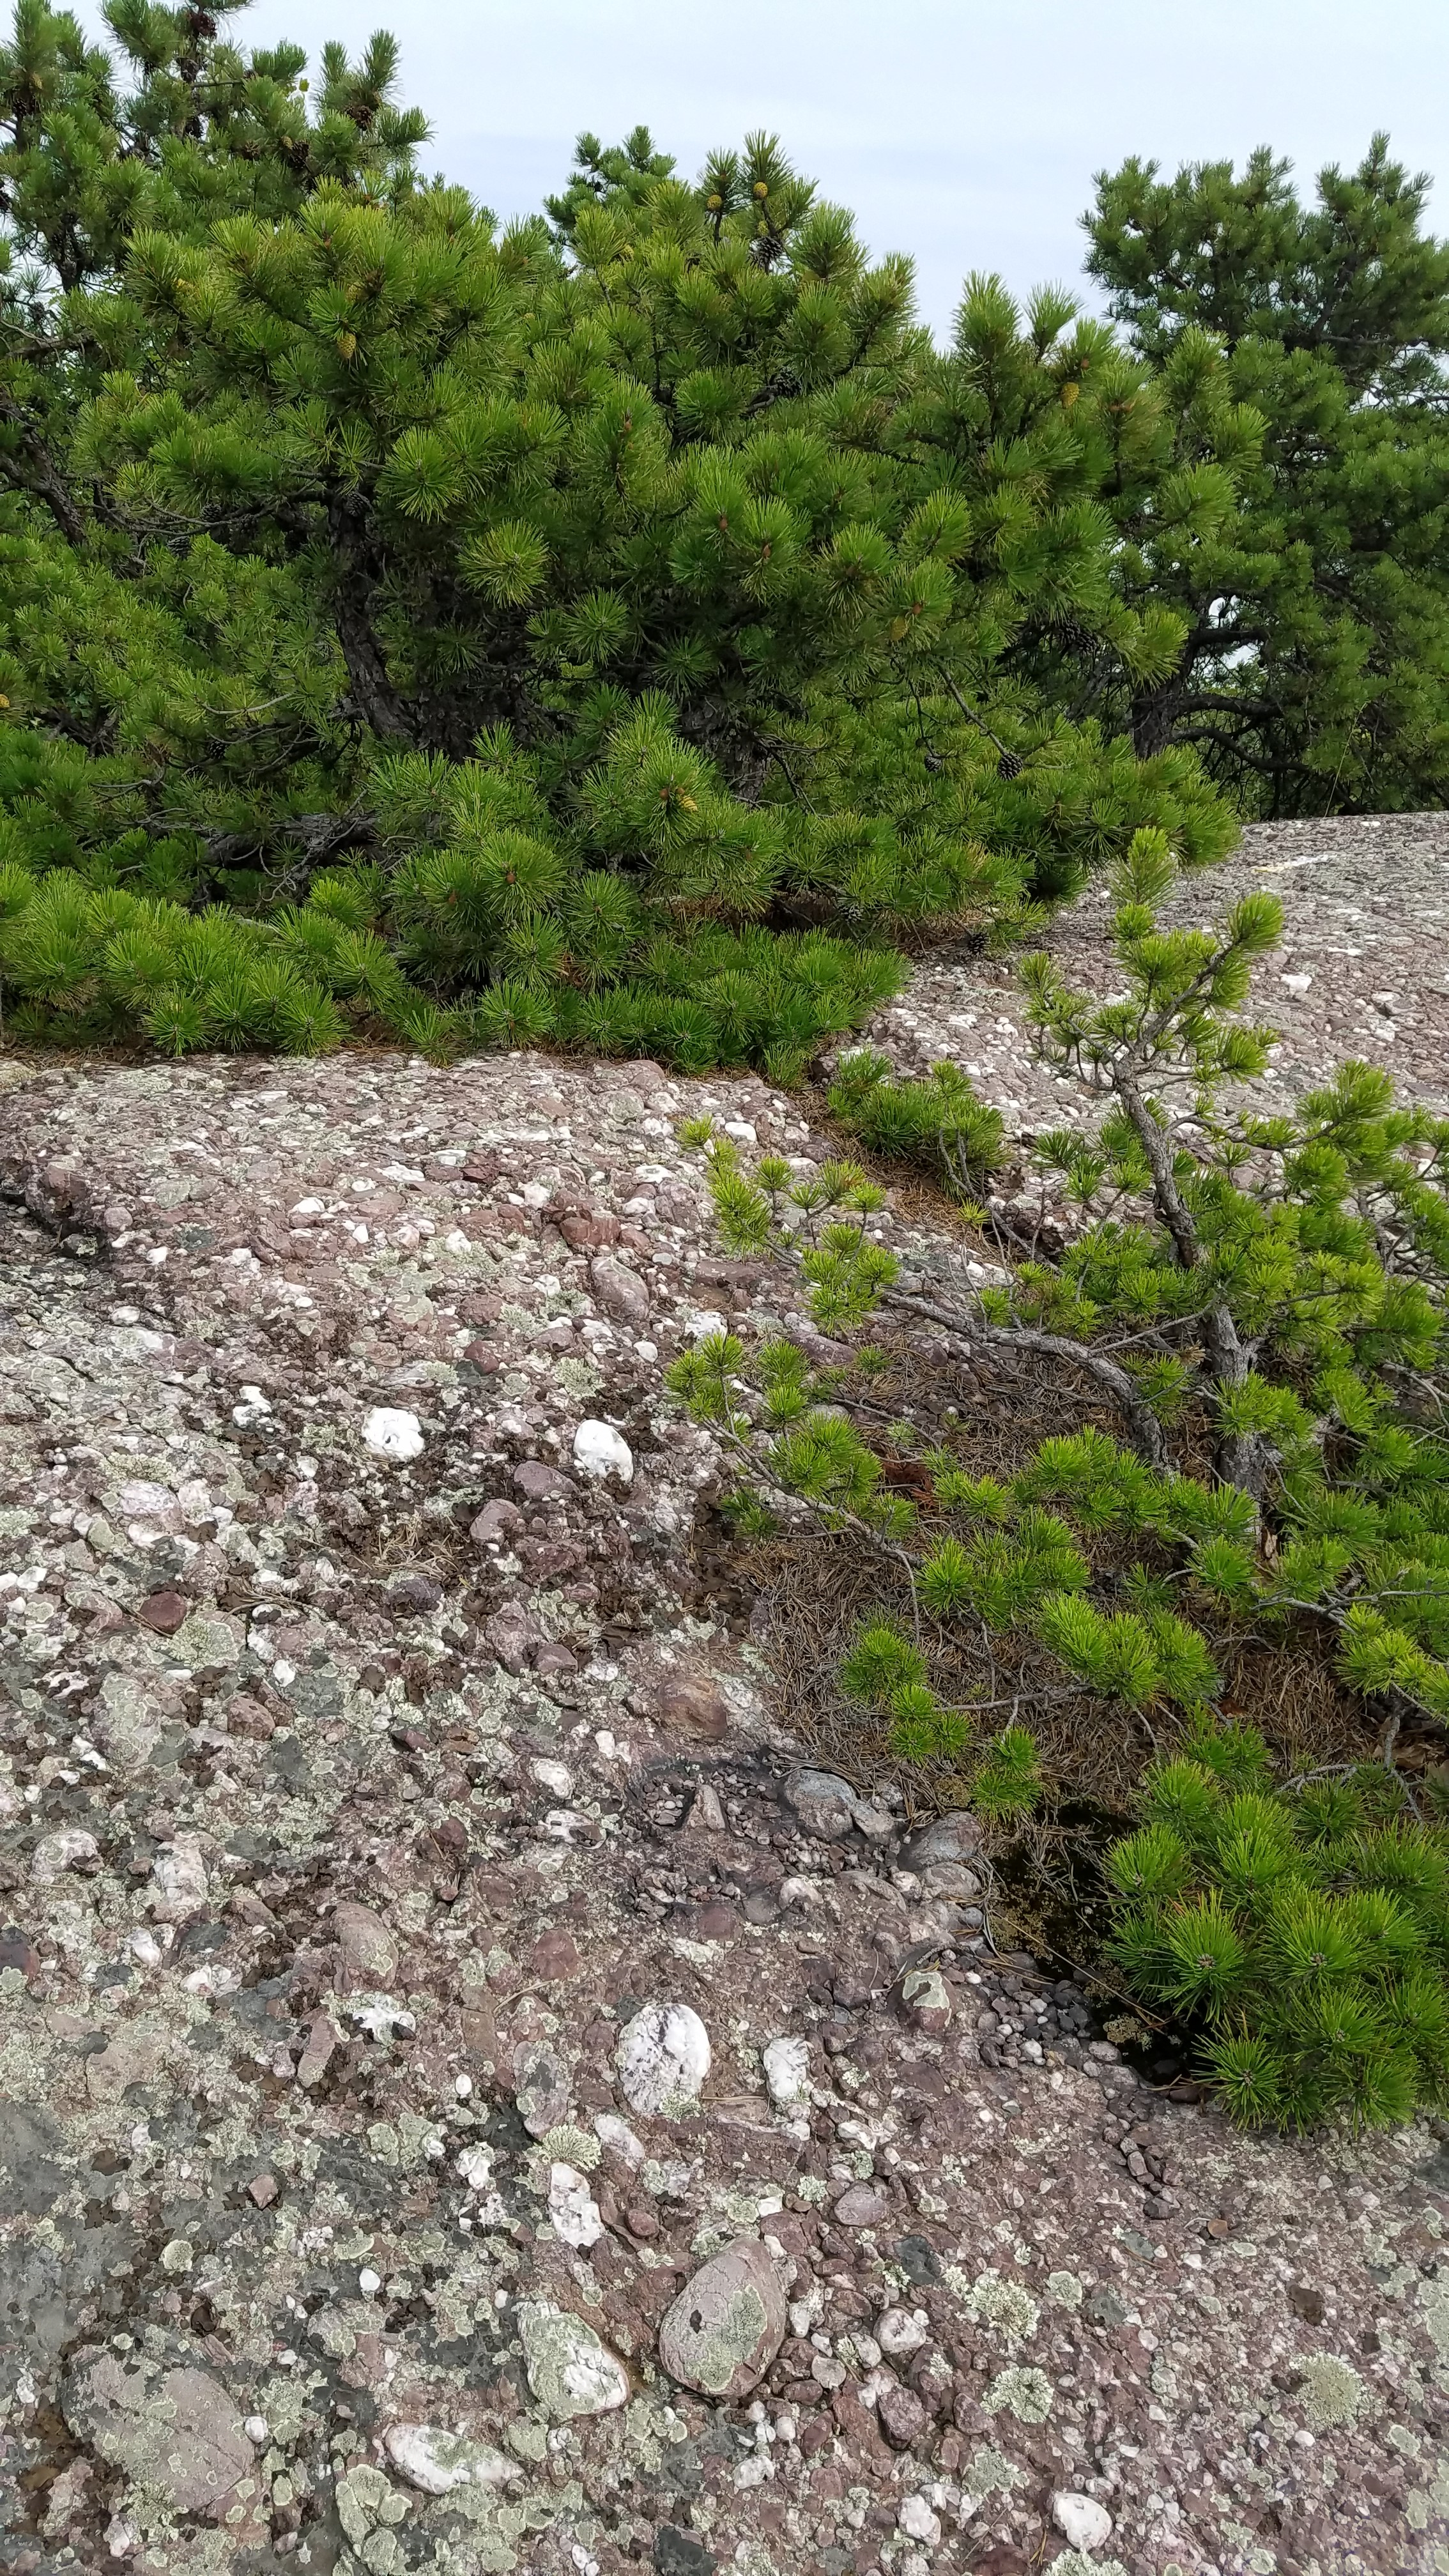
\includegraphics[width=0.4\textwidth]{images/Pudingstone.jpg}
        \caption{Schunnemunk Conglomerate (puddingstone)}\label{Schunnemunk Conglomerate}
\end{wrapfigure}
\begin{itemize}
    \item The southeast portion of Cornwall, which resides in the Hudson 
Highlands, is composed of undifferentiated gneiss, granite and granitic gneiss. 
Storm King Mountain is primarily composed of granite (granitic gneiss) and a 
small band of mafic gneiss.
    \item In the town's southwest, granite gives way to the Middle Devonian 
layered sandstone and shale of the Schunnemunk ridge.
  \item Much of the Town and Village’s more developed areas and commercial corridors 
    are underplayed by graywacke and shale bedrock within the Mount Merino and 
    Austin Glen formations (true?). The western part of the town north of 
    Schunnemunk Ridge is also mostly greywacke, shale, and siltstone.
    \item Significant portions of land on either side of the Moodna Creek are 
    underlayed by Quaternary alluvium and glacial drift
\end{itemize}
The surface of the bedrock varies in depth from surface exposure to greater 
than 100 feet deep. A report by the \gls{ocwa} found that 
wells drilled into bedrock units within the Town are not highly productive. 
Most residential wells within the Town are low yield bedrock wells. No high 
yield bedrock wells were identified during this study.

\paragraph{The Village of Cornwall on Hudson} has two main geologic features bisecting the 
Village: granitic gneiss and graywacke and shale. There is a small band of 
mafic gneiss in the southwest corner of the Village.

\subsection{Steep Slopes}\label{subsec:steepsloes}
\subsection*{Why you need this map}
The topic of steep slopes is an important consideration for municipalities when 
planning development of any kind. Steep slopes will also determine the physical 
limitations of development within a given municipality. The major concerns 
around slopes are erosion and flooding, which both impact the integrity of the 
natural and built environments around them. Trees and other vegetation hold the 
soils in place and can mitigate the effects of rain and wind on steeply sloped 
terrain. Allowing development or otherwise disturbing these areas makes soil 
unstable and more prone to erosion, and can have unintended adverse impacts on 
structures, roads, and natural and man-made drainage systems. In addition to 
posing a hazard to nearby structures and transportation corridors, the erosion 
of steep slopes can also greatly impact water quality, as loosened soil is 
washed into streams increasing water turbidity and sediment deposition. Any 
pollutants present in slope soil will also be spread into drainage systems in 
this fashion. This has the potential to negatively impact surface drinking 
water sources.

Steep slopes are valuable resources and are notable for their scenic and 
environmental qualities, which can bring special character to a community. 
Ravines and steep hillsides often provide scenic vistas, hiking opportunities, 
and natural beauty that can boost eco-tourism and property values. In many 
cases there is limited accessibility to steeply sloped terrain, and these areas 
provide vital undisturbed habitat for many plant and animal species. Steep 
slopes and cliffs can also form microclimates which can support unique and rare 
specimens of plants and animals. 

\begin{wrapfigure}{l}{0.6\textwidth}
    \hspace{-2mm}
        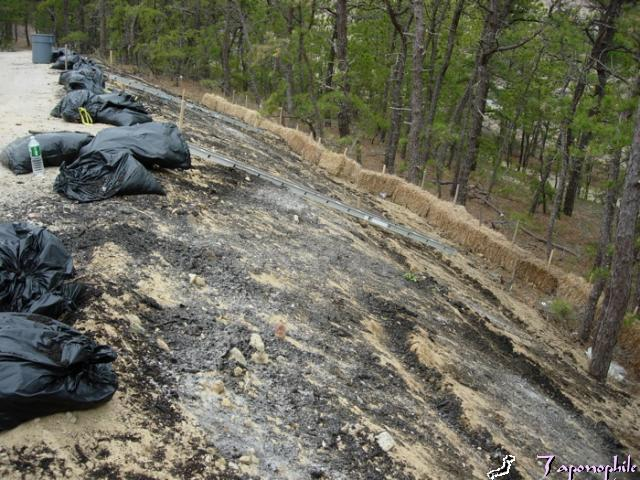
\includegraphics[width=0.5\textwidth]{images/compost222.jpg}
  %\caption{Watershed}
    \hspace{-2mm}
\end{wrapfigure}
The steepness of a slope is usually expressed as a percentage (rise over run). 
In general, the stability of slopes is determined by their grade and length, 
but also by their soil geology, amount of vegetative cover and the particular 
climate they are exposed to. Defining what constitutes “steep” for the purposes 
of slope regulation is at the discretion of each municipality, provided that the 
definition is reasonable. The USDA Natural Resources Conservation Service and 
numerous New York State municipalities more or less adhere to the following 
characterizations of steep slopes:

\begin{table}
\begin{center}
\begin{tabular}{ | p{0.2\textwidth} p{0.8\textwidth}| } 
\hline
Minor slopes < 8\% &
    \begin{itemize}
    \item Minor slopes are best suited for development and less costly to 
    develop; ponding, runoff, and erosion may be a problem on nearly level 
    slopes from 0-2 percent, unless the soils are well drained
    \item Erosion can occur on slopes as slight as 2-3 percent, depending on
    soils.
    \end{itemize}
    \\
\hline
Moderate Slopes 8-15\% &
    \begin{itemize}
        \item Present moderate septic problems because of possible seepage.
        \item Erosion potential exacerbated by the increase in grade
    \end{itemize}
    \\
\hline
Steep Slopes > 15\% (Very or Extremely Steep Slopes >25\%) &
    \begin{itemize}
    \item Slopes of 15\% and above are generally considered to be more 
    vulnerable to soil erosion, sedimentation, and other problems than more 
    gently sloping areas, with vulnerability increasing with steepness
    \item Slopes greater than 15 percent have soils that tend to be thin and 
    less fertile
    \item Many municipalities have significant land use restrictions for slopes 
    of over 15\%
    \item Construction on such areas can increase the sediment load of streams 
    100 fold
    \item Slopes of  >25\% should be left in a natural condition, carefully 
    maintained in grass or tree cover, or used as pastureland
    \end{itemize}
    \\
\hline
\end{tabular}
\end{center}
\caption{Adapted from \href{http://www.chathamtownship-nj.gov/images/CTEC/NRI1999/slopesadd090704.pdf}{Chatham Township Environmental Commission, 2014}\label{tab:steep_slopes}}
\end{table}
\subsection*{Steep Slopes Map}\label{subsec:steepslopes}
The slope designations on this map are broken down into three grades. Green 
indicates slopes of 8-15\%, yellow indicates slopes of 15.1-25\%, and red 
indicates slopes of greater than 25.1\%. The white areas are areas that are 
below 8\% of slope. A considerable amount of the land within Cornwall's borders 
is classified as steeply or very steeply sloped. The most significant areas of 
very steep slopes are encompassed within the borders of Schunnemunk Mountain 
State Park, Storm King State Park, and the Black Rock Forest Consortium. 
Outside the borders of these protected areas, however, there are numerous areas 
of steep slopes within both the town and village borders. Paired with the USDA 
NRC slope concerns mentioned above, municipal planning officials should 
primarily concern themselves with the yellow and red areas on this map when 
making decisions about land development or tree and vegetation removal.

Significant portions of the Village of Cornwall-on-Hudson are also 
characterized by steeply or very steeply sloped terrain. Residential areas 
along Mountain, Maple, and Deer Hill Roads as well as the Boulevard are 
potentially impacted by the slope considerations discussed in the chart above. 
The bluffs overlooking the Hudson River to the East account for the remainder of 
the steeply sloped land in the Village and erosion is currently a problem in 
certain areas where road and residential development exists. Other steeply 
slopes areas in the Town of Cornwall are mainly to be found bordering the Moodna 
Creek and along the residential corridor of Angola, Mine Hill, and Mineral 
Springs Roads. There are locations along the Moodna Creek where significant 
erosion due to the slope of the land and proximity to the creek has occurred. 
These areas will continue to pose a challenge to future town governments, 
departments, and planning boards.

It should be noted that the town of Cornwall zoning code currently considers 
slopes of >25\% to be inappropriate for development. However, given the 
challenges of increased erosion from heavier rain events due to climate change, 
the town should consider revisiting this criterion. Many municipalities have a 
steep slope zoning overlay as part of their general zoning code. Cornwall's 
existing Ridge Preservation zoning overlay focuses only on the largely 
undeveloped, mountainous terrain within the town’s borders. Given that 
significant parts of the town and village outside of that overlay are steeply 
sloped, Cornwall should consider developing a steep slope overlay to ensure 
careful consideration and management of development in these areas. For more 
information regarding recommendations for zoning, see the ~\nameref{subsec:zoning}
in this NRI.

\includepdf[pages=-,fitpaper]{cornwall_maps/SteepSlopes.pdf}\label{map:steepslopes}

\subsection{Soils}\label{subsec:soils}
\subsection*{Why you need these maps}
Familiarity with the characteristics and different classes of soil is an 
essential starting point to understanding the natural processes that influence 
our environment, and soil information both drives and reflects the uses imposed 
on it by human activities. Whether a soil is acidic or alkaline, loamy, sandy, 
clayey, deep or shallow defines its natural functions. It is important to 
consider these characteristics when a municipality is considering development 
and conservation plans. Soils function to regulate and filter water flow, 
decompose vegetative matter and other wastes, provide nutrients for agriculture, 
and support infrastructure. Soil data can play an important role in agriculture 
and forestry, as it tells us what plants can grow in a certain area and what 
level of irrigation and fertilization they may need. \textbf{Specific soil 
properties are critical factors to consider in land use planning: whether it is 
appropriate or feasible to build, whether septic systems or other types of 
wastewater treatment can or must be utilized, or how much surface area should be 
left in a permeable state}. They can also dictate whether certain building or 
foundation materials would be subject to corrosion by the pH character of the 
surrounding soil. 

\begin{wrapfigure}{l}{0.7\textwidth}
    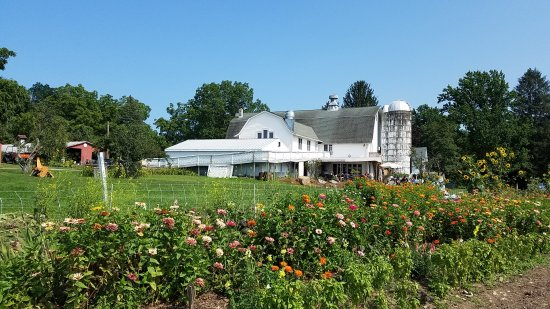
\includegraphics[width=0.6\textwidth]{images/asdasd.jpg}
  \caption{Watershed}
\end{wrapfigure}
Once polluted or depleted, soils can require long periods of 
replenishment/remediation or, worse, need to be abandoned. Recent studies have 
shown that soils, particularly adjacent to roadways, are vulnerable to salt and 
other chemical and heavy metal runoff. Depending on drainage characteristics, 
nearby streams and other bodies of water can also be impacted to the detriment 
of their dependent organisms. Stormwater drainage infrastructure can slow the 
degradation of soils adjacent to roadways as well. Run off from cold weather 
treatments for road surfaces is increasingly being recognized as a threat to 
soil quality adjacent to roads and can impact water quality of nearby streams 
and lakes. It is appropriate for municipalities to consider alternative 
treatments for road surfaces. 

In cases where soil quality creates areas of prime agricultural value or 
supports habitat for rare or endangered species, it may be determined that these 
areas are valuable enough that they should not be subject to commercial or 
residential development.

\includepdf[pages=-,fitpaper]{cornwall_maps/GeneralSoilClasses.pdf}\label{map:generalsoilclasses}

\subsection*{General Soil Classes Map}\label{subsec:generalsoil}
The General Soil Classes map focuses on the relative agricultural utility of 
the soils in our area. These classifications are determined by criteria set by 
the U.S. Department of Agriculture. There are a number of small patches of 
Areas of Prime Farmland (Pink) and Prime Farmland If Drained (Purple) within 
the borders of Cornwall, often contiguous to each other. These soils possess 
the most ideal combination of physical and chemical characteristics for 
producing agricultural products and growing feed for livestock. Looking at the 
~\nameref{map:calcaerousandglacialoutwashsoils}, we see that there is often a 
correlation between prime farmland and the presence of glacial outwash which 
consists of fertile soil material, as well as sand and gravel which aid in 
drainage.

Soils of Statewide Importance (Green) do not meet the criteria for Prime 
Farmland (or Prime Farmland if Drained), but still possess significant mineral 
loads that can support agriculture under the right conditions. Looking at the 
~\nameref{map:calcaerousandglacialoutwashsoils}, we see a correlation between these 
soils of statewide significance and the presence of calcareous and somewhat 
calcareous soils.

There are two very small deposits of black dirt/organic soil (Grey) in Cornwall, 
located in sector B2 on the ~\nameref{map:generalsoilclasses}. These soils are highly 
fertile and contain high levels of organic matter and chemical nutrients. The 
dominant soil class shown on the ~\nameref{map:generalsoilclasses} map, however, is 
Non-Agricultural (Yellow). These areas are predominantly located in and around 
the mountainous and rocky areas of Storm King and Schunnemunk Mountain state 
parks and ridgelines of Black Rock Forest where the soil coverage is 
comparatively shallow. It should be noted that much of the areas identified as 
Prime Farmland, Prime Farmland if Drained, and Soils of Statewide Importance are 
generally the location of residential and light commercial development within 
the Town. The Town should consider identifying any undeveloped prime farmland 
that may remain and prioritizing it for preservation or agricultural use. See 
the ~\nameref{map:landcover} chapters in this NRI for more detail.

\includepdf[pages=-,fitpaper]{cornwall_maps/CalcareousandGlacialOutwashSoils.pdf}
\label{map:calcaerousandglacialoutwashsoils}
\subsection*{Calcareous and Glacial Outwash Soils Map}\label{subsec:calcareous}
The soil types in the Cornwall/Cornwall-on-Hudson region are dominated by silt, 
rock outcrops, gravel, and gravelly silt. These soils result from glacial till 
deposits and together form a drainage sequence from the excessively drained, 
mountainous soils, to the poorly drained silts. The ~\nameref{map:calcaerousandglacialoutwashsoils}
map shows that, in Cornwall, the Calcareous (magenta) and Somewhat 
Calcareous (Yellow) soils, with their potential to provide habitats for rare 
species, are located throughout the lowland areas of the Town and Village. These 
areas are also characterized as “Soils of Statewide Importance” which means they 
also have agricultural value even though they do not meet the criteria for prime 
farmland and prime farmland if drained.

In geological terms, calcareous soils are those which contain a high proportion 
of calcium carbonate in the form of calcite or aragonite (limestone). 
Calcareous, or alkaline, soils serve as a habitat for a broad diversity of 
organisms and are often associated with uncommon habitats and rare species. 
Given their relatively high pH (7.5 to 8.4) they are not ideal for most 
agricultural uses. Somewhat Calcareous soils can have a pH as low as 6.5, and 
can function as agricultural land with the introduction of manure and other 
nitrogen-rich soil additives.